
\section{Subsistema de procesamiento de datos} \label{subsisdata}
\subsection{Procesamiento de ``Raw Data''}
\subsubsection{Input Data}

Los datos y/o señales de entrada para  el microcontrolador son los datos primarios (``Raw Data''), es decir que son valores sensados en tiempo real que no han sido modificados ni procesados manual o electrónicamente. Estos datos son obtenidos mediante los lectores RFID, las celdas de carga y los sensores de detección por infrarrojos de la Sección \ref{subsissen}.

\subsubsection{Output Data}

Los datos de salida son los datos entregados al usuario después de haber sido procesados. Esto hace referencia a los datos registrados en la base de datos que servirán como herramienta para monitorear la evolución alimenticia del ganado.

\subsection{Registro}

El registro de los datos se realiza mediante la programación de módulos de texto y generación de archivos con extensiones ``\texttt{.txt}'' y/o ``\texttt{.csv}''. Los datos adquiridos son anexados y acumulados después de haber sido adquiridos y procesados en sus respectivas etapas. Esto se realiza con el objetivo de llevar una trazabilidad de los datos. Así estos pueden ser analizados y aportar significativamente en la toma de decisiones de los productores ganaderos.

Los datos que se registren estarán separados por comas `` \texttt{,} ''. Estos datos son separados de esta forma por motivos convencionales de análisis de datos en herramientas computacionales para representación gráfica de datos como Excel. De esta forma se pueden crear Matrices de datos con filas y columnas correspondientes a los datos adquiridos durante la etapa de ingesta del ciclo iterativo del proceso de Ceba.

En cuestiones del prototipo de este proyecto, los datos son almacenados en memorias MicroSD y registrados en archivos de texto con extensión ``\texttt{.txt}''.

\pagebreak

% \subsubsection{Generación de archivos ``*.csv''}
\subsection{Comportamiento lógico del sistema}
\subsubsection{Diagrama de Contexto}

De manera similar al diagrama de bloques donde se definen las entradas, proceso y salidas del sistema o subsistemas, mediante este diagrama se definen los límites entre el sistema, y su ambiente, mostrando las entidades que interactúan con él. De esta forma se representan las entidades externas que pueden interactuar con el sistema. Estas entidades, son los elementos externos que interactúan con el sistema de cómputo o sistema de software (procesadores, controladores, etc).
Para este proyecto el sistema requiere de los elementos ubicados a los extremos laterales de la Figura \ref{contextopng}.\\
En el centro se encuentra el ``cerebro'' del sistema siendo el microcontrolador el encargado de procesar los datos de entrada y ejecutar las respectivas salidas. Se puede apreciar que algunas líneas cuentan con trazo continuo o entrecortado. Esta dependen del tipo de datos que se envían entre las entidades. Las lineas de trazo continuo son datos discretos o continuos, mientras que las de trazo entrecortado son señales de activación.

% \vspace{-35}

\begin{figure}[H]
    \begin{center}
    	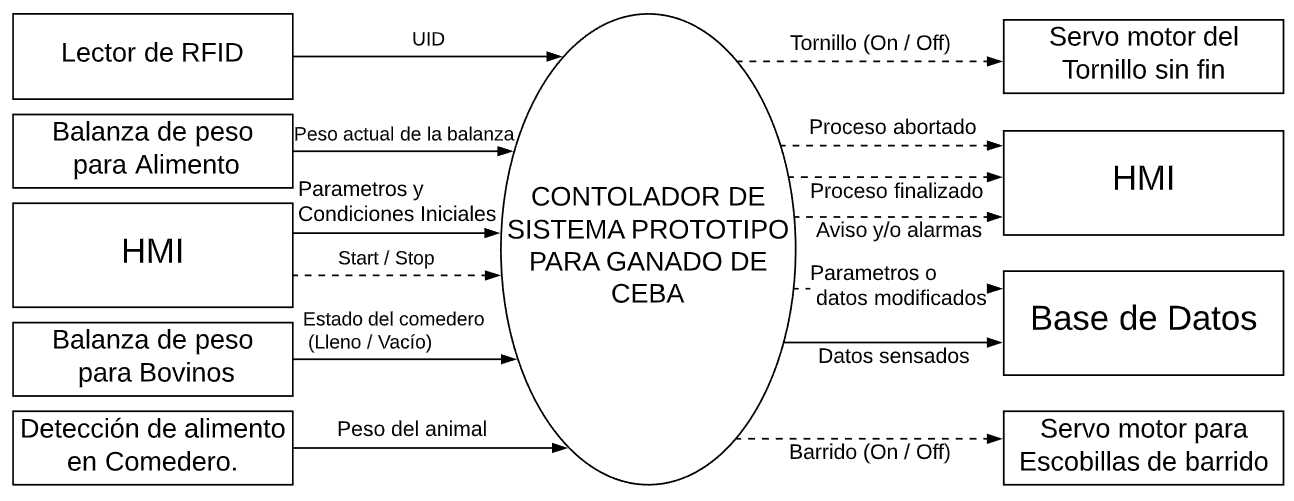
\includegraphics[scale=0.60]{img/contexto.png}
    \end{center}
    \caption{Diagrama de Contexto.}
    \label{contextopng}
\end{figure}

% \vspace{-45}
% \pagebreak

\subsubsection{Diagrama de estímulos}
Así como las máquinas y diagramas de estados son herramientas para comprender la evolución de los estados a partir de las entradas,
% Así Una manera simplificada para representar el comportamiento del sistema es mediante diagramas o maquinas de estados. De esta manera los cambios de estados o etapas pueden ser asimilados de manera simplificada y menos ambigua.
de forma similar, se puede representar la evolución lógica del sistema y sus entidades, mediante tablas de estímulos y transformaciones como la que se muestra a continuación:
\begin{table}[H]
    \centering
    \caption{Tabla de estímulos y transformaciones}
    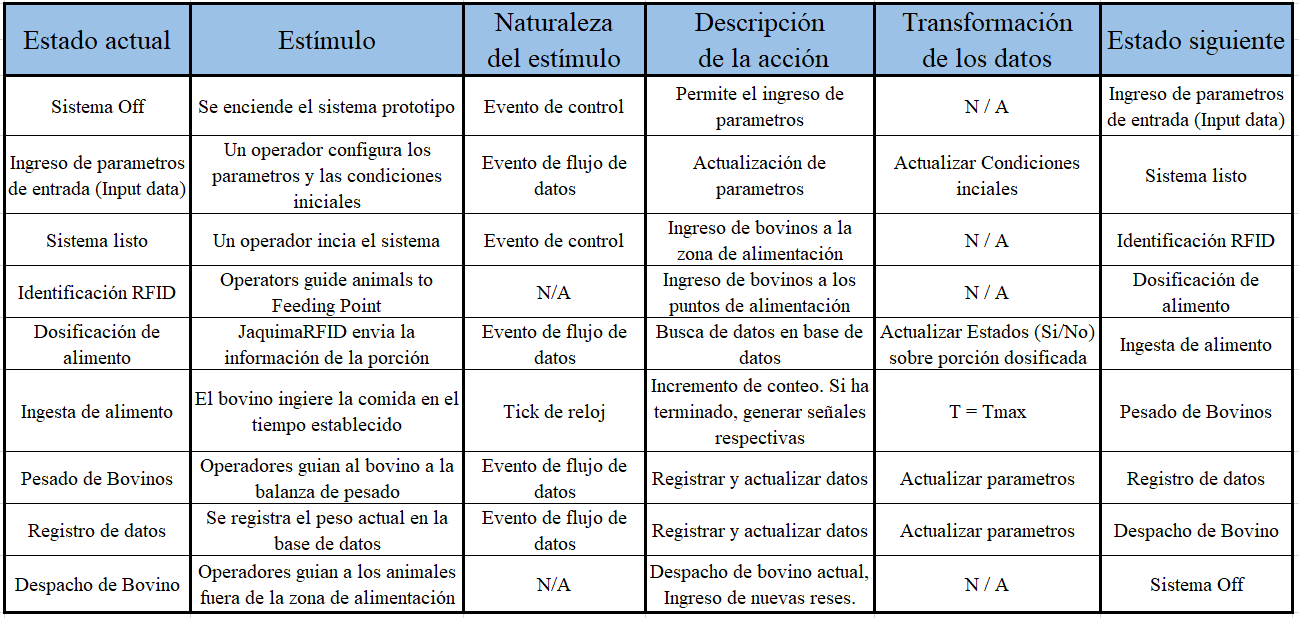
\includegraphics[scale=0.60]{img/estimulos.png}
\end{table}

%%% Tek

% \subsubsection{MSC}
% \subsubsection{SDL}

\subsubsection{Arquitectura}

Con el objetivo de simular un funcionamiento del sistema que evidencie situaciones cercanas a una implementación completa y real se considera un diseño lógico del comportamiento del sistema mediante la herramienta de software PragmaDev Studio. De esta forma se pueden organizar los procesos, canales de conexión y señales de comunicación entre los procesos.

Para este proyecto se diseña una arquitectura compuesta por un controlador, 11 procesos y un total de 33 señales de intercomunicación. Es importante aclarar que los procesos pueden ser usados por una misma entidad en diferentes cantidades que requieran del mismo proceso.

Esto quiere decir que para una implementación con 3 tolvas y 12 reses como se planteó en las consideraciones usadas para la Ecuación \ref{ecuaminima2} en la Sección \ref{subsissen}, no es necesario definir 12 procesos por cada RFID de cada bovino sino uno solo que aplique para las 12 reses. \\

\textbf{Los procesos \texttt{p[NombreProceso]} y los canales \texttt{c[NombreCanal]} pertenecientes a esta arquitectura son los siguientes:}
\begin{enumerate}
    % \begin{multicol}
    \item \texttt{pController}, como el proceso que representa al controlador.
    \item \texttt{pDatabase}, como el proceso que representa a la base de datos.
    \item \texttt{pRFIDsen}, en representación de los sensores lectores de RFID.
    \item \texttt{pBovineWSen}, en representación de la báscula de pesaje de bovinos.
    \item \texttt{pFoodWSen}, en representación de la báscula de pesaje de alimento.
    \item \texttt{pFoodPlateSen}, en representación de la detección de alimento en el comedero.
    \item \texttt{pFoodInTankSen}, en representación de la detección de alimento en la tolva.
    \item \texttt{pBrushHardware}, en representación del motor actuador de las escobillas de barrido fin.
    \item \texttt{pEndlessHardware}, en representación del motor actuador del tornillo sin.
    \item \texttt{pAlarmHardware}, en representación de las alarmas de interacción con el usuario.
    % \end{multicol}
% \end{enumerate}
% \pagebreak

% \textbf{Los canales de comunicación son los siguientes:}

% \begin{enumerate}
    % \begin{multicol}
    \item \texttt{cEnvCtrl}, Canal de comunicación entre el Controlador y el entorno
    \item \texttt{cCtrlRFID}, Canal de comunicación entre el Controlador y el lector RFID
    \item \texttt{cCtrlFoodWSen}, Canal de comunicación entre el Controlador y la báscula de pesaje de alimento
    \item \texttt{cCtrlPlate}, Canal de comunicación entre el Controlador y los sensores infrarrojos de detección de alimento en el comedero
    \item \texttt{cCtrlEnd}, Canal de comunicación entre el Controlador y el motor actuador del tornillo sin fin
    \item \texttt{cCtrlBase}, Canal de comunicación entre el Controlador y la base de datos
    \item \texttt{cCtrlBovineWSen}, Canal de comunicación entre el Controlador y la báscula de pesaje de bovinos
    \item \texttt{cCtrlTank}, Canal de comunicación entre el Controlador y la tolva
    \item \texttt{cCtrlBrush}, Canal de comunicación entre el Controlador y el motor actuador de las escobillas de barrido
    \item \texttt{cCtrlAlarm}, Canal de comunicación entre el Controlador y el actuador de la(s) alarma(s).
    % \end{multicol}
\end{enumerate}
\pagebreak


%\begin{figure}[H]
\begin{figure}
    \begin{center}
    	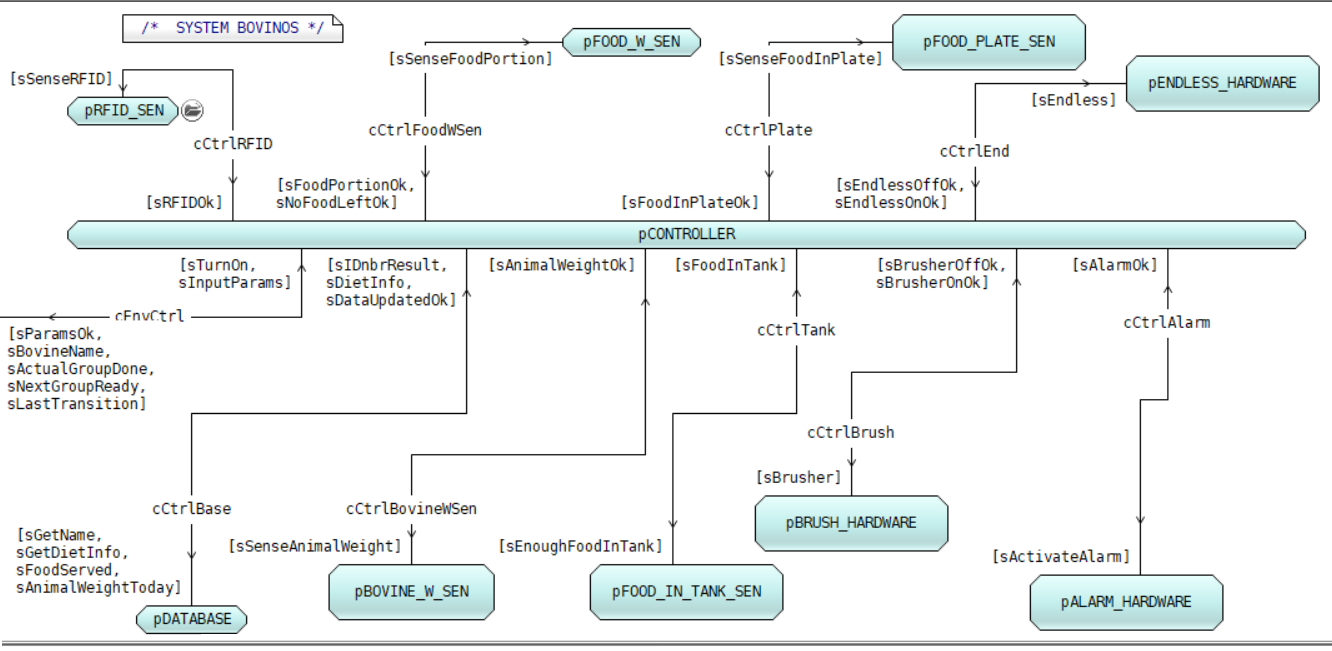
\includegraphics[scale=0.50,angle=90]{img/arqui.png}
    \end{center}
    \caption{Arquitectura, canales y señales de comunicación lógica del sistema prototipo.}
    \label{arquipng}
\end{figure}
%\pagebreak

\textbf{Las señales de interacción entre los procesos, el controlador y el entorno son las siguientes:}

\begin{figure}[H]
    \begin{center}
    	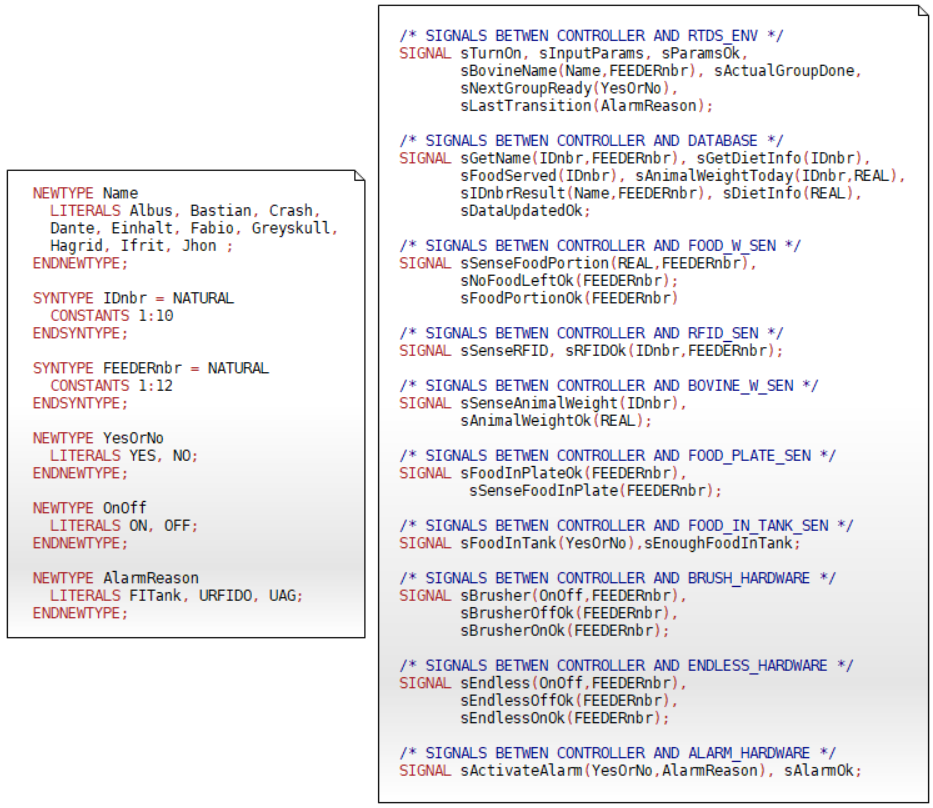
\includegraphics[scale=0.8]{img/senales2.png}
    \end{center}
    \caption{Tipos de señales de interacción entre los procesos, el controlador y el entorno}
    \label{senalespng}
\end{figure}

Con esto dicho, se procede a mostrar la arquitectura en la Figura \ref{arquipng}.

% \begin{itemize}
%     \item \textbf{Señales entre el Controlador y el Entorno}
%     \item \textbf{Señales entre el Controlador y la Base de datos}
%     \item \textbf{Señales entre el Controlador y la báscula de pesaje de alimento}
%     \item \textbf{Señales entre el Controlador y el lector RFID}
%     \item \textbf{Señales entre el Controlador y la báscula de pesaje de bovinos}
%     \item \textbf{Señales entre el Controlador y }
%     \item \textbf{Señales entre el Controlador y }
%     \item \textbf{Señales entre el Controlador y }
%     \item \textbf{Señales entre el Controlador y }
%     \item \textbf{Señales entre el Controlador y }
%     \item \textbf{Señales entre el Controlador y }
%     \item \textbf{Señales entre el Controlador y }
%     \item \textbf{Señales entre el Controlador y }
%     \item \textbf{Señales entre el Controlador y }
% \end{itemize}

%     \textbf{Bitácora del tiempo de PIPE 16/11/19:}
%     \textbf{xxx---   ----   ------   ---------   --------   -----xxx}
%     \textbf{xxx---   ----   ------   ---------   --------   -----xxx}
%     \textbf{Me falta:    Lo de la HMI \lonrightarrow{} PREGUNTAR A TAMURA.}
%     \textbf{xxx---   ----   ------   ---------   --------   -----xxx}
%     \textbf{xxx---   ----   ------   ---------   --------   -----xxx}

% \subsection{``Human-Machine Interface'' (HMI)}
% \subsubsection{Funciones}
% \subsubsection{FUNCIONES BASICAS (UNA A UNA)}
% \subsubsection{DISEÑO}
